\section{Auswertung}
\label{sec:Auswertung}

Im Folgenden wurden die baubedingten Fehler sämtlicher Bauteile vernachlässigt und 
treten somit auch nicht in den Fehlerrechnungen auf. Diese beschränken sich lediglich auf 
die Berechnung der Mittelwerte, sowie die damit verbundenen Fehler der Standartabweichungen.


\subsection{Wheatstonesche Brücke}
\label{WheatstonescheBrücke}

Mit den verwendeten Widerständen, die in Tabelle \ref{tab:1} aufgeführt werden, 
lassen sich durch Gleichung \ref{eq:1} folgende Werte für den 
unbekannten Widerstandswert $R_{11}$ berechnen:

\begin{align}
R_{11,1} = 491,821\,\si{\ohm} \nonumber \\
R_{11,2} = 492,794\,\si{\ohm} \nonumber \\
R_{11,3} = 490,313\,\si{\ohm} \nonumber 
\end{align}

\noindent
Über die zuvor aufgeführten Gleichungen \ref{eq:2} und \ref{eq:5} lassen sich der  
Mittelwert 

\begin{equation}
\bar{R_{11}} = 491,643\,\si{\ohm}, \nonumber
\end{equation}

\noindent
samt zugehörigem Fehler der Standartabweichung

\begin{equation}
\Delta R_{11} = 0,722\, \si{\ohm} \nonumber
\end{equation}

\noindent 
ermitteln.

\noindent
Das zusammengefasste Ergebnis für den, mithilfe der Wheatstoneschen Brückenschaltung, berechneten Widerstandswert
lautet demnach

\begin{equation}
R_{11} = (491,643 \pm 0,722)\,  \si{\ohm}. \nonumber
\end{equation}
    
\begin{table}[H]
\normalsize

\centering
\sisetup{table-format=4.0}
\begin{tabular}{c c c c}
\toprule
        Messung & $R_{2} \,/\,\si{\ohm}$ & $R_{3} \,/\,\si{\ohm}$ & $R_{4} \,/\,\si{\ohm}$ \\
        \midrule
        1 & 332 & 597 & 403  \\
        2 & 664 & 426 & 574  \\
        3 & 1000 & 329 & 671 \\ 
        
\bottomrule

\end{tabular}

\caption{Aufgenommene Werte zur Bestimmung von $R_{11}$}
\label{tab:1}
\end{table}







\subsection{Kapazitätsmessbrücke}
\label{Kapazitätsmessbrücke}

Unter Verwendung der oben ausgeführten Gleichungen \ref{eq:3} und \ref{eq:4}, sowie der aufgenommenen
Messwerte aus Tabelle \ref{tab:2}, können die Werte 
\begin{align}
R_{15,1} = 538.899\,\si{\ohm} \nonumber \\
R_{15,2} = 474.937\,\si{\ohm} \nonumber  
\end{align}
\\
für den ohmschen Widerstand und
\begin{align}
C_{15,1} = 491.625\,\si{\nano\ohm} \nonumber \\
C_{15,2} = 629.986\,\si{\nano\ohm} \nonumber 
\end{align}
\\
für die Kapazität des Kondensators in der RC-Kombination Nummer 15 ermittelt werden.
Mithilfe der Gleichungen \ref{eq:2} und \ref{eq:5}
lässt sich 
\begin{align}
R_{15} = (506.918 \pm 50.566)\, \si{\ohm} \nonumber 
\end{align}
\\
und
\begin{align}
C_{15} = (560.806 \pm 67.181)\, \si{\nano\farad} \nonumber 
\end{align}
\\
als Mittelwert samt Fehler der Standartabweichung für den ohmschen Widerstand beziehungsweise der
Kapazität der RC-Kombination Nummer 15 benennen.
\\
Im Folgenden setzt sich die RC-Kombination aus dem Kondensator Nummer 3 und dem Widerstand Nummer 10 zusammen. Weiterhin 
können die in Tabelle \ref{tab:3} aufgeführten Messwerte verwendet werden, um über die Gleichungen
\ref{eq:3} und \ref{eq:4}
\begin{align}
R_{10,1} = 239.429\, \si{\ohm} \nonumber
\end{align}
\\
als ohmschen Widerstand von Bauteil Nummer 10 und
\begin{align}
C_{3,1} = 553.267\, \si{\nano\farad} \nonumber
\end{align}
\\
als Kapazität des Bauteils Nummer 3 zu identifizieren. Da nur eine Messung durchgeführt wurde, können lediglich $R_{10,1}$
und $C_{3,1}$ angegeben werden, nicht aber Mittelwerte beziehungsweise Fehler der Standartabweichungen.


\begin{table}[H]
\normalsize

\centering
\sisetup{table-format=4.0}
\begin{tabular}{c c c c c}
\toprule
        Messung & $R_{2} \,/\,\si{\ohm}$ & $R_{3} \,/\,\si{\ohm}$ & $R_{4} \,/\,\si{\ohm}$ & $C_{2} \,/\, \si{\farad}$ \\
        
        \midrule
        1 & 664 & 448 & 552 & \num{399e-9} \\
        2 & 664 & 417 & 583 & \num{450e-9} \\

\bottomrule

\end{tabular}

\caption{Aufgenommene Werte zur Bestimmung von $R_{15}$ und $C_{15}$}
\label{tab:2}
\end{table}


\begin{table}[H]
\normalsize

\centering
\sisetup{table-format=4.0}
\begin{tabular}{c c c c c}
\toprule
        Messung & $R_{2} \,/\,\si{\ohm}$ & $R_{3} \,/\,\si{\ohm}$ & $R_{4} \,/\,\si{\ohm}$ & $C_{2} \,/\, \si{\farad}$ \\
        
        \midrule
        3 & 332 & 419 & 581 & \num{399e-9} \\

\bottomrule

\end{tabular}

\caption{Aufgenommene Werte zur Bestimmung von $R_{10}$ und $C_{3}$ } 
\label{tab:3}
\end{table}
















\subsection{Induktivitätsmessbrücke}
\label{Induktivitätsmessbrücke}

Für diesen Teil des Versuchs können die Werte aus Tabelle \ref{tab:4} und die Gleichungen
\ref{eq:6} und \ref{eq:7} verwendet werden, sodass die Ergebnisse der Einzelmessungen die Werte

\begin{align}
R_{18,1} = 3184.100\, \si{\ohm} \nonumber \\
R_{18,2} = 1130.555\, \si{\ohm} \nonumber \\
R_{18,3} = 2114.243\, \si{\ohm} \nonumber 
\end{align}
\\
für den Verlustwiderstand $R_{18}$ und
\begin{align}
L_{18,1} = 46.448\, \si{\milli\henry} \nonumber \\
L_{18,2} = 49.717\, \si{\milli\henry} \nonumber \\
L_{18,3} = 46.488\, \si{\milli\henry} \nonumber 
\end{align} 
\\
für die Induktivität $L_{18}$ der LR-Kombination liefern. Unter der Zuhilfenahme von Gleichungen
\ref{eq:2} und \ref{eq:5} lassen sich $R_{18}$ und $L_{18}$ durch ihre Mittelwerte und Fehler der Standartabweichungen
\begin{align}
R_{18} = (2142.966 \pm 592.981)\, \si{\ohm} \nonumber \\
L_{18} = (47.564 \pm 1.076)\, \si{\henry} \nonumber 
\end{align}
\\ 
angeben.

\begin{table}[H]
\normalsize

\centering
\sisetup{table-format=4.0}
\begin{tabular}{c c c c c}
\toprule
        Messung & $R_{2} \,/\,\si{\ohm}$ & $R_{3} \,/\,\si{\ohm}$ & $R_{4} \,/\,\si{\ohm}$ & $L_{2} \,/\, \si{\henry}$ \\
        \midrule
        1 & 1000 & 761 & 239 & \num{14.6e-3} \\
        2 & 332 & 773 & 227 & \num{14.6e-3} \\
        3 & 664 & 761 & 239 & \num{14.6e-3} \\
\bottomrule
\end{tabular}
\caption{Aufgenommene Werte zur Bestimmung von $R_{18}$ und $L_{18}$} 
\label{tab:4}
\end{table}




















\subsection{Maxwell-Brücke}
\label{MaxwellBrücke}

Um den Verlustwiderstand $R_{18}$, sowie die Induktivität $L_{18}$, der LR-Kombination ein weiteres Mal zu errechnen, sollen
nun die Werte aus Tabelle \ref{tab:5} und die beiden Gleichungen \ref{eq:12} und \ref{eq:13} verwendet werden. Somit
ergeben sich für $R_{18}$
\begin{align}
R_{18,1} = 208.000\, \si{\ohm} \nonumber \\
R_{18,2} = 204.000\, \si{\ohm} \nonumber \\
R_{18,3} = 204.819\, \si{\ohm} \nonumber 
\end{align}.
\\Ein analoges Vorgehen ergibt
\begin{align}
L_{18,1} = 51.792\, \si{\milli\henry} \nonumber \\
L_{18,2} = 50.796\, \si{\milli\henry} \nonumber \\
L_{18,3} = 51.000\, \si{\milli\henry} \nonumber 
\end{align}
\\ 
als Werte für $L_{18}$. Daran geschlossen können die beiden gesuchten Größen unter Verwendung von Gleichung
\ref{eq:2} und \ref{eq:5}
über die Mittelwerte der Messungen, sowie den Fehler der Standartabweichung angegeben werden. Folglich ergibt sich
\begin{align}
R_{18} = (205.606 \pm 1.220)\, \si{\ohm} \nonumber
\end{align}
\\
für den Verlustwiderstand $R_{18}$ und
\begin{align}
L_{18} = (51.196 \pm 0.304)\, \si{\milli\henry} \nonumber
\end{align}
\\
für die Induktivität $L_{18}$ der LR-Kombination.

\begin{table}[H]
\normalsize
\centering
\sisetup{table-format=4.0}
\begin{tabular}{c c c c c}
\toprule
        Messung & $R_{2} \,/\,\si{\ohm}$ & $R_{3} \,/\,\si{\ohm}$ & $R_{4} \,/\,\si{\ohm}$ & $C_{4} \,/\, \si{\farad}$ \\
        \midrule
        1 & 332 & 208 & 332 & \num{750e-9} \\
        2 & 664 & 102 & 332 & \num{750e-9} \\
        3 & 1000 & 68 & 32 & \num{750e-9} \\
\bottomrule
\end{tabular}
\caption{Aufgenommene Werte zur Bestimmung von $R_{18}$ und $L_{18}$} 
\label{tab:5}
\end{table}

\subsection{Frequenzabhängigkeit der Brückenspannung einer Wien-Robinsson-Brücke}

Um den Theoriewert für $\nu_{0}$ zu erhalten, muss zunächst $\omega_{0}$ mit 
\begin{align}
\omega_{0} = \frac{1}{R \cdot C} \nonumber
\end{align}
\\ 
berechnet werden. Durch Einsetzen der Größen, die in der Tabelle \ref{tab:6} 
aufgeführt sind, ergibt sich
\begin{align}
\omega_{0} = \frac{1}{1000\, \si{\ohm} \cdot 420\, \si{\nano\farad}} = 2380.952\, \si{\hertz} \nonumber
\end{align}
\\ 
als Kreisfrequenz. Nach Umrechnung der Kreisfrequenz $\omega_{0}$ in die Frequenz $\nu_{0}$ mithilfe von 
\begin{equation}
\nu_{0} = \frac{\omega_{0}}{2 \cdot \pi} \nonumber
\end{equation}
\\
ergibt sich der Theoriewert 
\begin{align}
\nu_{0} = \frac{2380.952\, \si{\hertz}}{2 \cdot \pi} = 378.94\, \si{\hertz} \nonumber
\end{align}
für die Kreisfrequenz, bei der die minimale Brückenspannung $U_{Br}$ gemessen werden kann.

In Abbildung \ref{fig:plot} wurden die Messwerte, ebenso wie die mit Gleichung \ref{eq:10}
berechneten Werte für die Theoriekurve, aufgetragen. Auf der x-Achse ist das Verhältnis $\Omega$ von $\nu$ zu $\nu_{0}$
logarithmisch aufgetragen, wohingegen die y-Achse das Verhältnis von der Brückenspannung $U_{Br}$ zu der Speisespannung
$U_{S}$ widergibt.
Es fällt auf, dass der prozentuale Fehler des gemessenen Wertes für $\nu_{0}$ mit 
\begin{align}
\upDelta_{p} \nu = 0.2789\, \% \nonumber
\end{align}
\\
gering ausfällt. Weiterhin ist zu beobachten, dass die Messwerte um das Frequenzverhältnis $\Omega = 1$
herum sehr nah an der Theoriekurve liegen. Allerdings vergrößtert sich die Abweichung von Theoriekurve zu den aufgenommenen
Messwerten zunächst, je weiter das Frequenzverhältnis von dem Wert eins abweicht. Für Frequenzverhältnisse, die sich dem Wert Null
annähert, ist zu beobachten, das Theoriekurve und Messwerte nicht weiter auseinanderlaufen. Im Gegensatz dazu lässt sich 
dieses Verhalten für Frequenzverhältnisse $\Omega > 0$ nicht beobachten.


\begin{figure}[h]
  \centering
  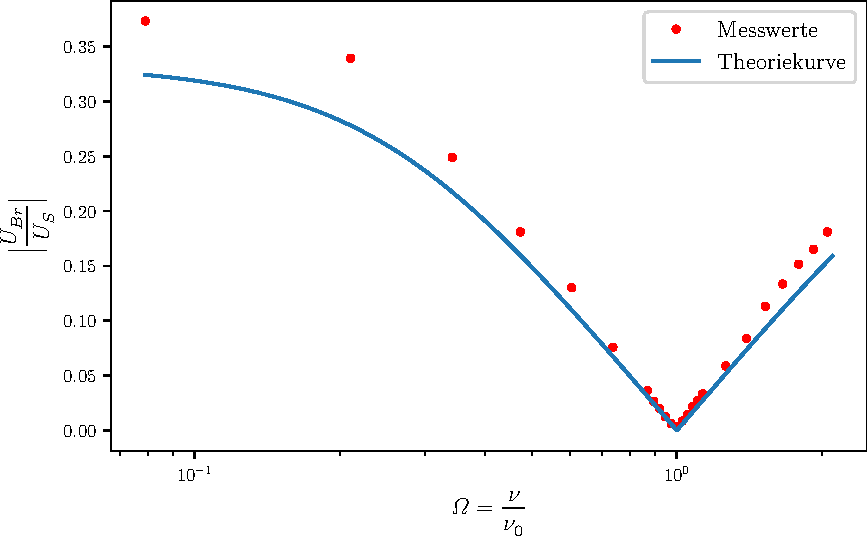
\includegraphics{plot.pdf}
   \caption{Darstellung der aufgenommenen Messwerte und der Theoriekurve}
   \label{fig:plot}
\end{figure}


\begin{table}[h]
\normalsize
\centering
\sisetup{table-format=4.0}
\begin{tabular}{c c c c}
\toprule
        $2R' \,/\,\si{\ohm}$ & $R' \,/\,\si{\ohm}$ & $R \,/\,\si{\ohm}$ & $C_{4} \,/\, \si{\farad}$ \\
        \midrule
        664 & 332 & 1000 & \num{420e-9} \\
\bottomrule
\end{tabular}
\caption{Aufgenommene Messwerte zur Bestimmung von $\nu_{0}$} 
\label{tab:6}
\end{table}


\begin{table}[h]
\normalsize
\centering
\sisetup{table-format=4.0}
\begin{tabular}{c c c c}
\toprule
        $U_{S} \,/\,\si{\milli\volt}$ & $U_{Br} \,/\,\si{\milli\volt}$ & $\upOmega$ & $\nu \,/\, \si{\henry}$ \\
        \midrule
        2500 & 1320 &           0.0789 & 30 \\
        2500 & 1200 &           0.2105 & 80 \\
        2500 & 880 &            0.3221 & 130 \\
        2500 & 640 &            0.4737 & 180 \\
        2500 & 460 &            0.6053 & 230 \\
        2500 & 268 &            0.7368 & 280 \\
        2500 & 128 &            0.8684 & 330 \\
        2500 & 94.4 &           0.8947 & 340 \\
        2500 & 70.4 &           0.9211 & 350 \\
        2500 & 44.0 &           0.9474 & 360 \\
        2500 & 21.6 &           0.9737 & 370 \\
        2500 & 13.6 &           1.0000 & 380 \\   
        2500 & 30 &             1.0263 & 390 \\
        2500 & 52 &             1.0526 & 400 \\
        2500 & 78 &             1.0789 & 410 \\
        2500 & 96 &             1.1053 & 420 \\
        2500 & 118 &            1.1316 & 430 \\
        2500 & 208 &            1.2631 & 480 \\
        2500 & 296 &            1.3947 & 530 \\
        2500 & 400 &            1.5263 & 580 \\
        2500 & 472 &            1.6579 & 630 \\
        2500 & 536 &            1.7894 & 680 \\
        2500 & 584 &            1.9210 & 730 \\
        2500 & 640 &            2.0526 & 780 \\
        
\bottomrule
\end{tabular}
\caption{Aufgenommene Messwerte zur Bestimmung des Klirrfaktors $k$} 
\label{tab:7}
\end{table}


\subsection{Klirrfaktormessung}

Zuletzt soll eine Näherung für den Klirrfaktor $k$ mit Gleichung \ref{eq:11} ermitteln werden, wobei 
davon ausgegangen werden soll, dass $U_{i} = 0\, \si{\volt}$ mit $i\,>\,2$ gilt.  

\noindent Dafür soll zunächst das Spannungsverhältnis $\lvert{\frac{U_{Br}}{U_S}}\rvert$ für $\Omega = 2$ ermittelt werden. Dieses ergibt sich 
durch Verwendung von Gleichung \ref{eq:10} und liefert 
\begin{align}
f(2) =  \frac{1}{9} \cdot \frac{(\Omega^2 - 1)^2}{(1 - \Omega^2)^2 + 9 \cdot \Omega^2}  = \frac{\sqrt{5}}{15} = \frac{1}{\sqrt{45}} \nonumber
\end{align}
\\
als Wert. Bevor der Klirrfaktor $k$ nun ermittelt werden kann, müssen zunächst die Amplituden $U_{1}$ und $U_{2}$ berechnet werden.
Die Amplitude der Grundwelle $U_{1}$ entspricht der Speisespannung $U_{S}$, von der bereits der Effektivwert gegeben ist, wohingegen die Amplitude $U_{2}$ der Spannung der
2-ten Oberwelle entspricht und für den vorliegenden Versuch mit Gleichung \ref{eq:8}
\begin{align}
U_{2} = \frac{9.6166\, \si{\milli\volt}}{\sqrt{\frac{1}{45}}} = 0.0645\, \si{\volt} \nonumber
\end{align}
\\
lautet. Der Effektivwert der Spannung wird mit 
\begin{align}
U_{2,eff} = \frac{U_{2}}{\sqrt{2}} = 0.0456\, \si{\volt} \nonumber
\end{align}
\\
errechnet.
Mit diesen Werten und Gleichung \ref{eq:8} ergibt sich 
\begin{align}
k = \frac{U_{2}}{U_{1}} = \frac{0.0456\, \si{\volt}}{2.5\, \si{\volt}} = 0.0182 \nonumber
\end{align}
\\ 
für den gesuchten Klirrfaktor $k$.